\newpage
\chapter{Introducción}

% Tema de investigación.
% Breve síntesis metodológica.
% Resumen de resultados.
% Potencial de impacto.
% Una visualización que sustente sus resultados.

\noindent  Este proyecto se realizó para participar en el \href{http://http://dataton.datos.gob.mx}{Datatón}.

Para empezar se puede ver que los delitos cometidos en Zapopan son principalmente delitos de incidencia. Sin 


\begin{figure}[H]
\centering
\caption{Delitos en Zapopan}
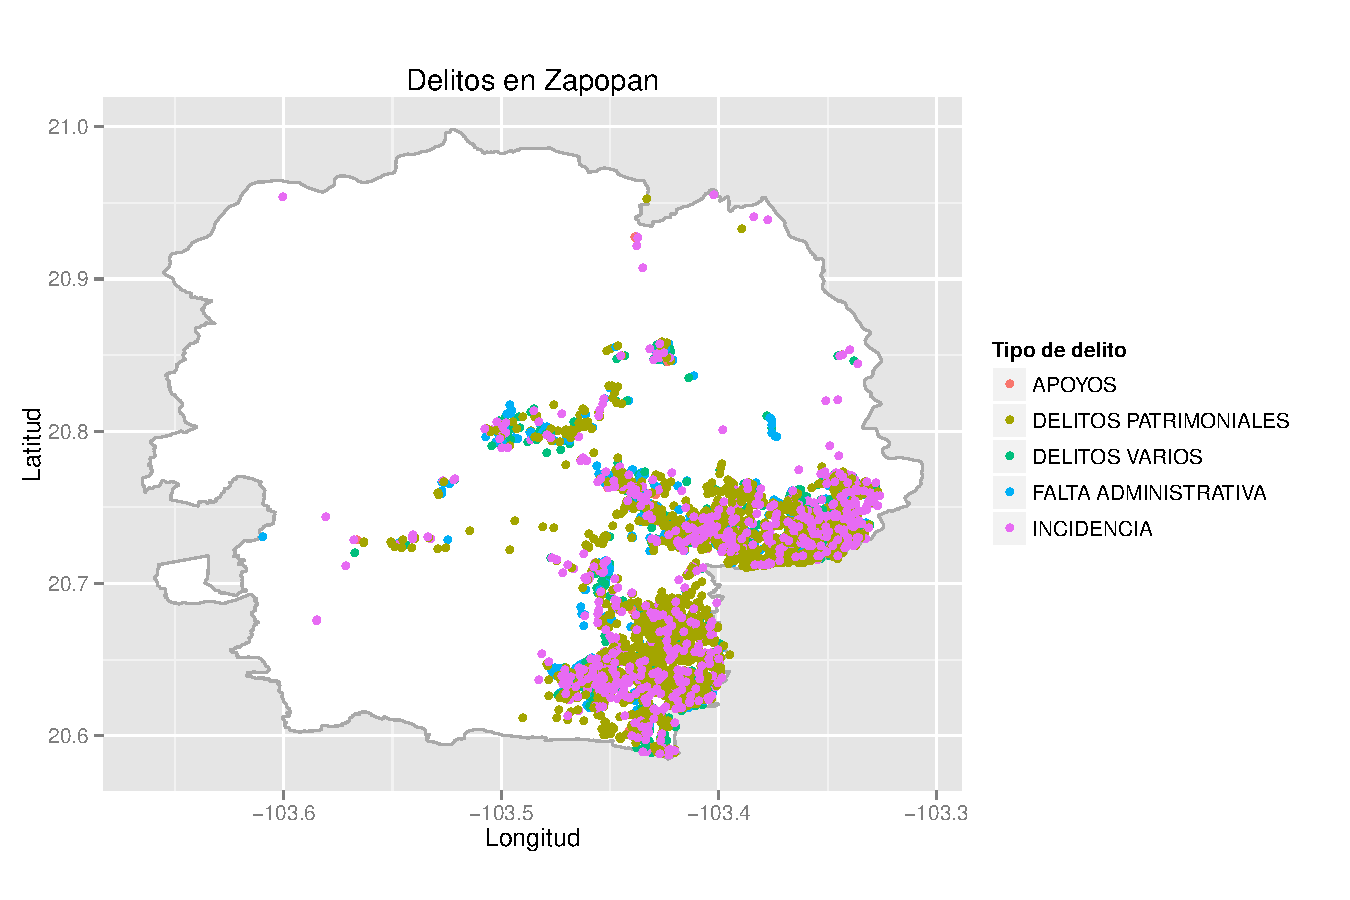
\includegraphics[width=120mm]{../../graphs/zapopan_delitos.pdf}
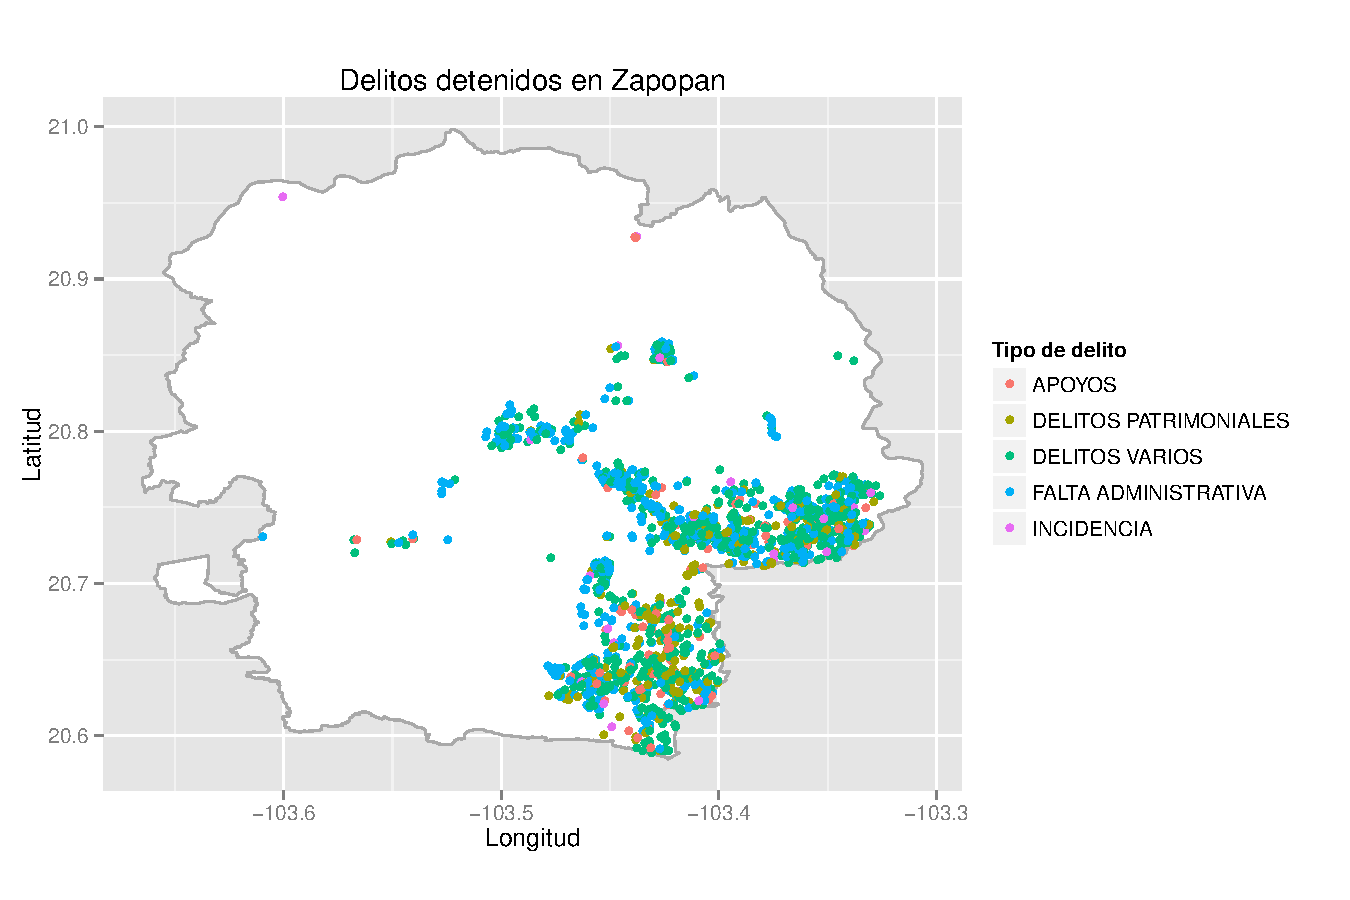
\includegraphics[width=120mm]{../../graphs/zapopan_delitos_detenidos.pdf}
\end{figure}


\begin{table}[H]
\centering
\caption{Número de delitos cometidos y detenidos} 
\begin{tabular}{lrr}
  \hline
Tipo de delito & Cometidos & Detenidos \\ 
  \hline
APOYOS & 101 & 131 \\ 
  DELITOS PATRIMONIALES & 2293 & 398 \\ 
  DELITOS VARIOS & 896 & 1158 \\ 
  FALTA ADMINISTRATIVA & 807 & 3215 \\ 
  INCIDENCIA & 789 &  29 \\ 
   \hline
\end{tabular}
\end{table}

\begin{table}[H]
\centering
\caption{Porcentaje de delitos cometidos y detenidos} 
\begin{tabular}{lrr}
  \hline
Tipo de delito & \% de cometidos & \% de detenidos \\ 
  \hline
APOYOS & 2 & 3 \\ 
  DELITOS PATRIMONIALES & 47 & 8 \\ 
  DELITOS VARIOS & 18 & 23 \\ 
  FALTA ADMINISTRATIVA & 17 & 65 \\ 
  INCIDENCIA & 16 & 1 \\ 
   \hline
\end{tabular}
\end{table}

\begin{table}[H]
\centering
\caption{Las 20 colonias más peligrosas} 
\begin{tabular}{rllr}
  \hline
 & Colonia & Tipo de delito & n \\ 
  \hline
1 & PASEOS DEL SOL & DELITOS PATRIMONIALES &  70 \\ 
  2 & TABACHINES & DELITOS PATRIMONIALES &  67 \\ 
  3 & SAN JUAN DE OCOTAN & FALTA ADMINISTRATIVA &  65 \\ 
  4 & ARBOLEDAS & DELITOS PATRIMONIALES &  57 \\ 
  5 & CALMA LA & DELITOS PATRIMONIALES &  49 \\ 
  6 & CABECERA MUNICIPAL & FALTA ADMINISTRATIVA &  45 \\ 
  7 & JARDINES VALLARTA & DELITOS PATRIMONIALES &  39 \\ 
  8 & SAN JUAN DE OCOTAN & DELITOS VARIOS &  39 \\ 
  9 & ESTANCIA LA & DELITOS PATRIMONIALES &  38 \\ 
  10 & MIRAMAR & DELITOS PATRIMONIALES &  38 \\ 
  11 & ARCOS DE ZAPOPAN & DELITOS PATRIMONIALES &  37 \\ 
  12 & COLLI EL & DELITOS PATRIMONIALES &  37 \\ 
  13 & CABECERA MUNICIPAL & DELITOS PATRIMONIALES &  36 \\ 
  14 & PARAISOS DEL COLLI & DELITOS PATRIMONIALES &  36 \\ 
  15 & AGUILAS LAS & DELITOS PATRIMONIALES &  34 \\ 
  16 & CONSTITUCION & DELITOS VARIOS &  33 \\ 
  17 & CONSTITUCION & DELITOS PATRIMONIALES &  29 \\ 
  18 & ARENALES TAPATIOS & DELITOS VARIOS &  28 \\ 
  19 & CABECERA MUNICIPAL & DELITOS VARIOS &  28 \\ 
  20 & CAMICHINES VALLARTA & DELITOS PATRIMONIALES &  26 \\ 
   \hline
\end{tabular}

\end{table}
